\section{Audio}
\label{sec:audio}
The audio system is is responsible for playing sfx and music.
\begin{itemize}
    \item Sfx work in a 'fire and forget' way: a single function call to the AudioSource is required to start playing the sound, and it never needs to be stopped or cleaned up in any way. The engine stops playing the sfx when it is finished \footnote{Unless specified that the sound should loop}.
    \item Music can be played, stopped and adjusted while it is playing, however, just like sfc, music does not need to be manually stopped.
\end{itemize}

\subsection{Audio library}
As discussed in the research, it is best to use an audio library (rather than manually doing system calls)
, and there are many audio libraries to choose from. By trying out various audio libraries, it was concluded that
SDL Mixer is the best library to use for this engine. While it is not as extensive as other libraries,
it has the features to meet the engine requirements, and its ease of use makes it a sensible choice.

\subsection{Class diagram}
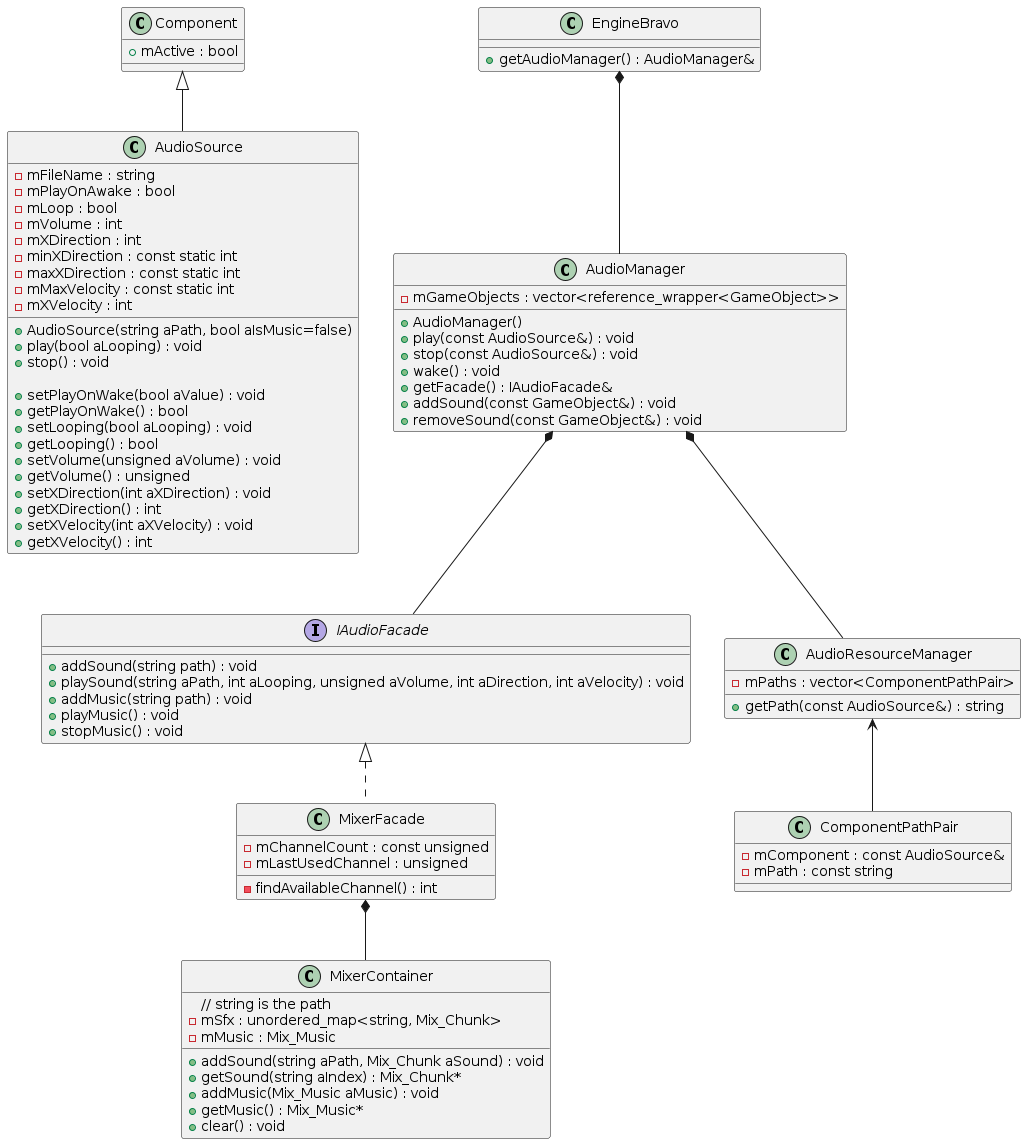
\includegraphics[width=\textwidth]{audioClassDiagram.png}
In the following subsections, the classes in this diagram are further detailed.
\subsubsection{AudioSource}
The AudioSource is a class required by the project's API, it is one of the child classes of Component.
It will therefore be owned by a GameObject, and represent either a single sfx or song.

Things to note about the AudioSource:
\begin{itemize}
    \item When creating an AudioSource, it must be explicitly stated if it is music or an sfx. This is because the AudioManager treats these differently.
    \item mPlayOnWake (required by API) indicates whether the audio source should be played when a new scene is loaded. When this is false, the audio only plays when play() is called.
    \item The x direction and velocity represent the location of the sound in the game, from left to right (x-axis).\footnote{Because the engine is made for 2D games, there is no depth (z-axis) members. Adding verticallity (y-axis) to sound is complex, and out of the scope of this project.} \footnote{The x coordinates and velocity are unrelated to the coordinate system for the game objects.}
\end{itemize}

\subsubsection{AudioManager}
The AudioManager is, similarly to the other manager classes, responsible for controlling all of the sound features in the engine.
It contains only a few basic methods, and delegates most functionality to the audio facade and audio resource manager.

\begin{itemize}
    \item The wake method is used to indicate when a new scene is loaded. This is used to play all the AudioSources set to play on wake.
    \item The mGameObjects contains references to all GameObjects which own an AudioSource. Each cycle, this list is updated by the EngineBravo (which owns the AudioManager), by calling addSound and removeSound. This way, the AudioManager does not have to manually check which objects do and do not own an audio source.
\end{itemize}

\subsubsection{AudioResourceManager}
The AudioResourceManager is intended to reduce the amount of memory the engine requires.
If the audio resource manager is not used, each game object with a sound source would load the required sound file.
When there are many game objects which all use the same sfx file, this file would be loaded into memory multpile times, which is inefficient.
To solve this, the audio resource manager is created. This class makes sure that for each path, only one sound file is loaded.
It makes use of the ComponentPathPair, to keep track of the relation between the AudioSource components and their paths.

\subsubsection{IAudioFacade}
A facade interface to make the coupling between the AudioManager and the used audio library less tight.

\subsubsection{MixerFacade}
The implementation of the audio facade interface for SDL mixer.
Because channel \footnote{what is called a channel in SDL mixer is more commonly known as a track.} management is done
manually in SDL mixer, the mChannelCount and mLastUsedChannel variables are used to determine the next available channel for playing sfx.

\subsubsection{MixerContainer}
The mixer container holds all the
SDL mixer sound files.
The string in the mSfx map is the path to the file, because that can be considered as a sort of unique id for the sound file.